\section{Remesアルゴリズムによる最良近似多項式の計算}
\label{sec:remes_algorithm}

本章では，第2章で述べた最良近似多項式の存在定理および交替定理に基づき，実際に最良近似多項式を数値的に求めるためのアルゴリズムであるRemesアルゴリズムについて説明する．
このアルゴリズムは，1934年にEvgeny Remesによって提案された反復解法であり，任意の連続関数に対して，交替定理の条件を満たす参照点を効率的に探索する手法である．

\subsection{アルゴリズムの概要と計算手順}
\label{subsec:algo_overview}

Remesアルゴリズムの基本的なアイデアは，区間 $[a, b]$ 内の $n+2$ 個の参照点 $\xi^{(k)} = \{x_0^{(k)}, x_1^{(k)}, \dots, x_{n+1}^{(k)}\}$ を初期設定し，反復ごとにこれを更新して，最終的に誤差関数の極値点と参照点が一致するように収束させることである．
特に，本研究では収束速度に優れる「全点同時入れ替え法」を採用する．

アルゴリズムの各ステップは以下の通りである．

\subsubsection{Step 0: 初期参照点の設定}
近似区間 $[a, b]$ 内に，$a \le x_0 < x_1 < \dots < x_{n+1} \le b$ を満たす $n+2$ 個の点を選び，初期参照点 $\xi^{(0)}$ とする．
初期値の選び方は任意であるが，収束を速めるために，通常はチェビシェフ多項式の極値点を区間 $[a, b]$ に写像した点が用いられる．

\subsubsection{Step 1: 近似多項式の導出（係数決定）}
現在の参照点 $\boldsymbol{\xi}^{(k)}$ 上で，誤差が交互に符号を変え，かつその絶対値が等しくなるような多項式 $P(x)$ と，その誤差の大きさ $E$ を決定する．
この $E$ は，現在の参照点集合 $\boldsymbol{\xi}^{(k)}$ の上でのみ成立する均等な誤差であり，これを\textbf{参照均等誤差}（levelled reference error）と呼ぶ\cite{seminar-note}．
具体的には，以下の連立方程式を解く．

\begin{equation}
    f(\xi_i) - P(\xi_i) = (-1)^i E \quad (i = 0, 1, \dots, n+1).
    \label{eq:remes_linear_system}
\end{equation}

ここで，$P(\xi) = \sum_{j=0}^n c_j \xi^j$ とおくと，式(\ref{eq:remes_linear_system})は係数 $c_0, \dots, c_n$ および $E$ を未知数とする $n+2$ 元の連立一次方程式となる．
これを行列形式で記述すると以下のようになる．

\begin{equation}
    \left(
    \begin{array}{ccccc}
    1 & \xi_0 & \dots & \xi_0^n & 1 \\
    1 & \xi_1 & \dots & \xi_1^n & -1 \\
    \vdots & \vdots & \ddots & \vdots & \vdots \\
    1 & \xi_{n+1} & \dots & \xi_{n+1}^n & (-1)^{n+1}
    \end{array}
    \right)
    \left(
    \begin{array}{c}
    c_0 \\
    c_1 \\
    \vdots \\
    c_n \\
    E
    \end{array}
    \right)
    =
    \left(
    \begin{array}{c}
    f(\xi_0) \\
    f(\xi_1) \\
    \vdots \\
    f(\xi_{n+1})
    \end{array}
    \right).
\end{equation}

この方程式をLU分解で解くことで，現在の参照点集合に対する「最良近似」となる多項式 $P(x)$ が一意に定まる．

\subsubsection{Step 2: 誤差関数の極値探索}
求めた多項式 $P(x)$ に対する誤差関数 $e(x) = f(x) - P(x)$ を定義し，区間 $[a, b]$ 全体における極値を探索する．
具体的には，$e(x)$ の極大値・極小値を与える点，および区間の端点の中から，誤差の絶対値 $|e(x)|$ が現在の均等誤差 $|E|$ よりも大きくなる点を探し出す．

もし，すべての $x \in [a, b]$ において $|e(x)| \le |E| + \varepsilon$ （$\varepsilon$ は許容誤差）が成り立つならば，現在の $P(x)$ は最良近似多項式であるとみなしてアルゴリズムを終了する．

\subsubsection{Step 3: 参照点の更新（全点同時入れ替え）}
Step 2 で見つけた極値点を用いて，次の参照点 $\xi^{(k+1)}$ を決定する．
新しい参照点集合は，交替定理の条件（誤差の符号が交互になること）を維持しつつ，各点での誤差の絶対値ができるだけ大きくなるように選ばれる．

一般的には，誤差関数 $e(x)$ の零点を境界として区間を分割し，各部分区間内で $|e(x)|$ が最大となる点を新しい参照点 $x_i^{(k+1)}$ として採用する．
これにより，参照点は真の最良近似における極値点へと近づいていく．

\subsection{Remesアルゴリズムの収束性}
\label{subsec:remes_convergence}
対象関数 $f(x)$ が区間 $[a, b]$ 上で十分に滑らか（$C^2$級以上）であり，かつ最良近似多項式の誤差関数が正常な数（ちょうど $n+2$ 個）の極値を持つ場合，
全点同時入れ替え法を用いたRemesアルゴリズムは2次収束することが知られている．
本節では，このアルゴリズムがニュートン法によってそれが保証される事を示し，その収束性を理論的に説明する．
なお，本節の議論は参考文献\cite{seminar-note}に基づく．

\subsubsection{最良近似問題の非線形方程式への帰着}

対象関数 $f(x)$ が区間 $[a, b]$ 上で2回連続微分可能であり，その最良近似多項式 $P^*(x)$ の誤差関数 $e^*(x) = f(x) - P^*(x)$ が，区間内部にちょうど $n+1$ 個の極値を持つ（端点を含めて $n+2$ 個の偏差点を持つ）と仮定する．

このとき，最良近似多項式を決定するために求めるべき未知数は，以下の3組である．
\begin{itemize}
  \item 多項式の係数ベクトル $\boldsymbol{c} = (c_0, \dots, c_n)$ \quad ($n+1$ 個)
  \item 最大誤差（均等誤差） $E$ \quad ($1$ 個)
  \item 偏差点列の座標ベクトル $\boldsymbol{\xi} = (\xi_0, \dots, \xi_{n+1})$ \quad ($n+2$ 個)
\end{itemize}
これら合計 $2n+4$ 個の変数は，以下の連立非線形方程式の解として特徴づけられる．

\begin{numcases}{}
  f(\xi_i) - \sum_{j=0}^n c_j \xi_i^j - (-1)^i E = 0 & $(i = 0, \dots, n+1).$ \label{eq:remes_nonlinear_1} \\
  f'(\xi_i) - \sum_{j=0}^n c_j j \xi_i^{j-1} = 0 & $(i = 1, \dots, n).$ \label{eq:remes_nonlinear_2}
\end{numcases}

式(\ref{eq:remes_nonlinear_1})は交替定理の条件（各点での誤差が $\pm E$ になること）を表し，式(\ref{eq:remes_nonlinear_2})は各点 $\xi_i$ が誤差関数の極値（微分係数が0）であることを表している（端点は固定とする）．

\subsubsection{Remesアルゴリズムとニュートン法との等価性と2次収束性}
\label{subsec:newton_equivalence}

Remesアルゴリズム（全点同時入れ替え法）の反復手順は，前節で導出した非線形方程式系 $\boldsymbol{F}(\boldsymbol{y}) = \boldsymbol{0}$ に対するニュートン法と構造的な対応関係にある．
具体的には，未知数ベクトル $\boldsymbol{y}$ の更新量 $\Delta \boldsymbol{y} = \boldsymbol{y}^{(k+1)} - \boldsymbol{y}^{(k)}$ は，ニュートン法の方程式
\begin{equation}
  \boldsymbol{J}(\boldsymbol{y}^{(k)}) \Delta \boldsymbol{y} = -\boldsymbol{F}(\boldsymbol{y}^{(k)})
  \label{eq:newton_step}
\end{equation}
によって決定されるが，Remesアルゴリズムはこれを以下の2段階に分離して実行していると解釈できる\cite{seminar-note}．

\begin{enumerate}
  \item \textbf{係数と誤差の更新（Step 1に対応）:}
  ニュートン法における係数ベクトル $\boldsymbol{c}$ および $E$ の更新は，方程式系(\ref{eq:remes_nonlinear_1})の線形部分を解くことに相当する．Remesアルゴリズムでは，現在の点 $\boldsymbol{\xi}^{(k)}$ を固定した状態でこの線形方程式を解いている．
  
  \item \textbf{偏差点の更新（Step 2に対応）:}
  偏差点 $\boldsymbol{\xi}$ の更新は，方程式系(\ref{eq:remes_nonlinear_2})すなわち誤差関数の導関数 $e'(x)=0$ の根を求めることに対応する．
  Remesアルゴリズムにおいて，現在の近似多項式 $P^{(k)}$ に基づいて新たな極値を探す操作は，幾何学的には誤差関数の勾配情報を用いた修正を行うことと同義であり，これはニュートン法における $\boldsymbol{\xi}$ 成分の更新ステップ
  \[ \xi_i^{(k+1)} \approx \xi_i^{(k)} - \frac{e'(\xi_i^{(k)})}{e''(\xi_i^{(k)})} \]
  を（高精度な探索によって）実行していることと等価である．
\end{enumerate}

参考文献\cite{seminar-note}によると，解の十分近傍において，このRemesアルゴリズムの手順はニュートン法の反復ステップと（高次の微小項を除いて）一致することが解析的に示されている．

ニュートン法は解の近傍において2次収束することが知られているため，Remesアルゴリズムにおいても，初期参照点 $\boldsymbol{\xi}^{(0)}$ が真の解 $\boldsymbol{\xi}^*$ に十分近ければ，誤差 $\delta_k = \|\boldsymbol{\xi}^{(k)} - \boldsymbol{\xi}^*\|$ は以下の不等式を満たす．

\begin{equation}
  \delta_{k+1} \le C \delta_k^2
\end{equation}

ここで $C$ は正の定数である．
すなわち，解の近傍では誤差が反復ごとに二乗で減少するため，収束が著しく高速となる．

\label{subsec:algo_implementation}
\subsection{アルゴリズムの実装と検証}
% =========================================================
% Goプログラム (remes_comparison.go) が生成した
% プロセス可視化ファイル（グラフと表）を読み込む
% =========================================================
%% 3章用 (Grid)

前述の理論に基づき，本研究ではGo言語を用いてRemesアルゴリズムを実装した．
以下の図表は，関数 $f(x) = \frac{1}{1+25x^2}$ ($n=15$) を近似した際の収束過程を示したものである．

表\ref{tab:remes-grid-log}は，各反復で算出された参照均等誤差 $|E|$ と，その時点での誤差関数の極値の絶対値の最大値と最小値の差（Deviation）の推移を示したものである．

本実装における収束判定条件は，すべてのパラメータの変化量が機械イプシロン（$\epsilon_{\text{mach}} \approx 2.22 \times 10^{-16}$）以下になった時点とする．
\begin{itemize}
  \item 近似多項式の係数ベクトル $\boldsymbol{c}$ の最大変化量：
  \[ \|\boldsymbol{c}^{(k+1)} - \boldsymbol{c}^{(k)}\|_\infty \le \epsilon_{\text{mach}}. \]
  \item 参照点ベクトル $\boldsymbol{\xi}$ の最大変化量：
  \[ \|\boldsymbol{\xi}^{(k+1)} - \boldsymbol{\xi}^{(k)}\|_\infty \le \epsilon_{\text{mach}}. \]
  \item 均等誤差パラメータ $E$ の変化量：
  \[ |E^{(k+1)} - E^{(k)}| \le \epsilon_{\text{mach}}. \]
\end{itemize}
これにより，数値計算上の限界精度まで解が収束したことを保証する．

表中の Deviation は，係数が収束に向かうにつれて交替定理の条件（等振幅性）が満たされていく様子を表す指標であり，理論通り急速に 0 に収束していることが確認できる．

図\ref{fig:remes-grid-convergence}は，この Deviation の推移を可視化したものである．
初期段階では不揃いであった誤差の波形が，最終的には振幅が一定の美しい等振動波形へと収束していることが見て取れる．

\begin{figure}[H]
 \centering
 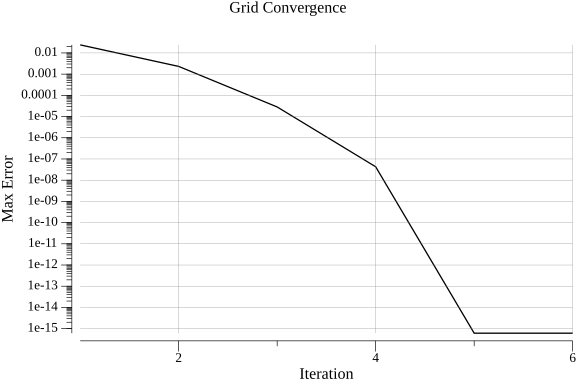
\includegraphics[width=0.6\linewidth]{material/remes/outputs/grid/convergence_grid.png}
 \caption{グリッド極値点探索法による最大誤差の収束履歴}
 \label{fig:remes-grid-convergence}
\end{figure}

\begin{figure}[H]
 \centering
 \begin{minipage}[b]{0.48\textwidth}
  \centering
  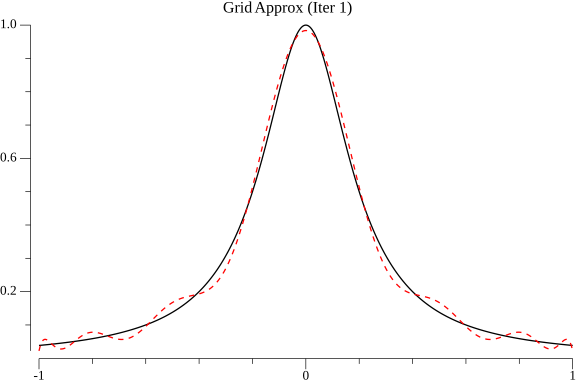
\includegraphics[width=1.0\linewidth]{material/remes/outputs/grid/func_remes_grid_iter01.png}
  \caption{Iter 1}
 \end{minipage}
 \hfill
 \begin{minipage}[b]{0.48\textwidth}
  \centering
  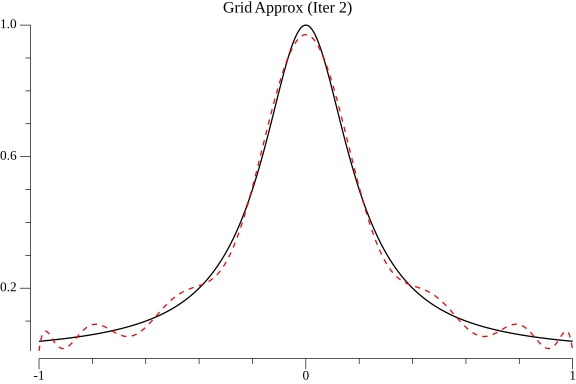
\includegraphics[width=1.0\linewidth]{material/remes/outputs/grid/func_remes_grid_iter02.png}
  \caption{Iter 2}
 \end{minipage}

 \begin{minipage}[b]{0.48\textwidth}
  \centering
  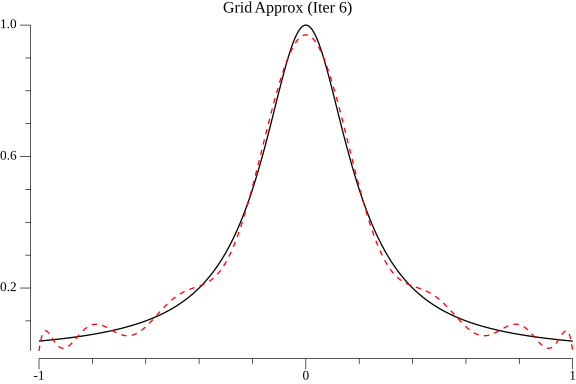
\includegraphics[width=1.0\linewidth]{material/remes/outputs/grid/func_remes_grid_iter06.png}
  \caption{Iter 6}
 \end{minipage}

 \caption{グリッド法: 近似多項式の推移}
 \label{fig:remes-grid-approx}
\end{figure}
\begin{figure}[H]
 \centering
 \begin{minipage}[b]{0.48\textwidth}
  \centering
  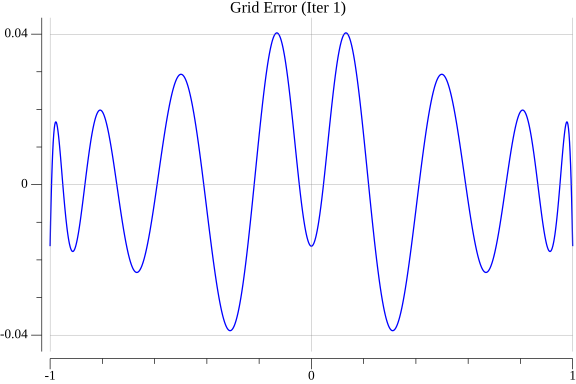
\includegraphics[width=1.0\linewidth]{material/remes/outputs/grid/error_remes_grid_iter01.png}
  \caption{Iter 1}
 \end{minipage}
 \hfill
 \begin{minipage}[b]{0.48\textwidth}
  \centering
  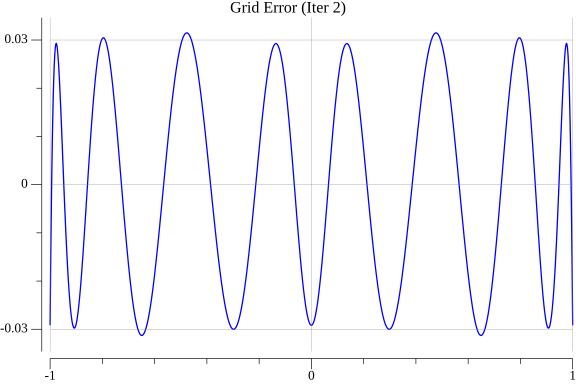
\includegraphics[width=1.0\linewidth]{material/remes/outputs/grid/error_remes_grid_iter02.png}
  \caption{Iter 2}
 \end{minipage}

 \begin{minipage}[b]{0.48\textwidth}
  \centering
  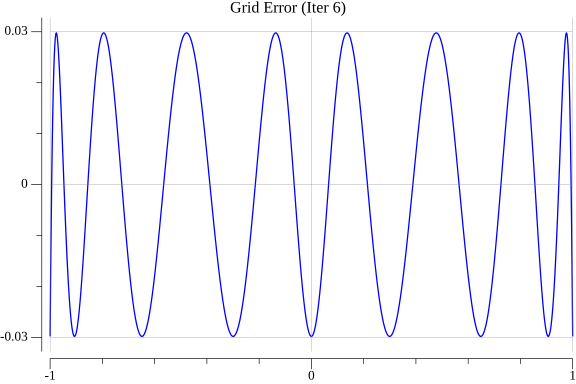
\includegraphics[width=1.0\linewidth]{material/remes/outputs/grid/error_remes_grid_iter06.png}
  \caption{Iter 6}
 \end{minipage}

 \caption{グリッド法: 誤差関数の推移}
 \label{fig:remes-grid-error}
\end{figure}

\begin{table}[H]
 \centering
 \caption{グリッド極値点探索法の収束ログ}
 \label{tab:remes-grid-log}
 \begin{tabular}{crrrr}
 \toprule
 Iter & $|E|$ & Coeff Norm & Node Move & Error Change \\
 \midrule
 1 & $1.63552e-02$ & $0.00000e+00$ & $0.00000e+00$ & $0.00000e+00$ \\
 2 & $2.91689e-02$ & $1.37847e-02$ & $4.92138e-02$ & $1.28137e-02$ \\
 3 & $2.97722e-02$ & $1.25091e-03$ & $3.16228e-03$ & $6.03335e-04$ \\
 4 & $2.97756e-02$ & $1.30728e-05$ & $1.41421e-03$ & $3.38844e-06$ \\
 5 & $2.97756e-02$ & $1.90384e-08$ & $0.00000e+00$ & $7.83719e-09$ \\
 6 & $2.97756e-02$ & $0.00000e+00$ & $0.00000e+00$ & $0.00000e+00$ \\
 \bottomrule
 \end{tabular}
\end{table}

\begin{table}[H]
 \centering
 \caption{グリッド極値点探索結果の等振幅性確認（節点近傍の偏差）}
 \label{tab:remes-grid-final-check}
 \begin{tabular}{crrr}
 \toprule
 No. & Grid誤差 & Brent誤差 & 差分 \\
 \midrule
 1 & $2.97755952e-02$ & $2.97755952e-02$ & $-6.86950e-16$ \\
 2 & $2.97755952e-02$ & $2.97755952e-02$ & $3.80066e-11$ \\
 3 & $2.97755952e-02$ & $2.97755952e-02$ & $1.63316e-11$ \\
 4 & $2.97755952e-02$ & $2.97755952e-02$ & $1.94925e-12$ \\
 5 & $2.97755952e-02$ & $2.97755952e-02$ & $4.93021e-12$ \\
 6 & $2.97755952e-02$ & $2.97755952e-02$ & $1.21936e-12$ \\
 7 & $2.97755952e-02$ & $2.97755952e-02$ & $4.76352e-12$ \\
 8 & $2.97755952e-02$ & $2.97755952e-02$ & $6.46216e-12$ \\
 9 & $2.97755952e-02$ & $2.97755952e-02$ & $0.00000e+00$ \\
 10 & $2.97755952e-02$ & $2.97755952e-02$ & $6.46216e-12$ \\
 11 & $2.97755952e-02$ & $2.97755952e-02$ & $4.76358e-12$ \\
 12 & $2.97755952e-02$ & $2.97755952e-02$ & $1.21927e-12$ \\
 13 & $2.97755952e-02$ & $2.97755952e-02$ & $4.93020e-12$ \\
 14 & $2.97755952e-02$ & $2.97755952e-02$ & $1.94927e-12$ \\
 15 & $2.97755952e-02$ & $2.97755952e-02$ & $1.63316e-11$ \\
 16 & $2.97755952e-02$ & $2.97755952e-02$ & $3.80066e-11$ \\
 17 & $2.97755952e-02$ & $2.97755952e-02$ & $-1.34615e-15$ \\
 \bottomrule
 \end{tabular}
\vspace{1mm}

\small \textbf{注：}
\small 上表は，区間 $[-1.0,1.0]$ を探索するRemesアルゴリズムによって導かれた誤差関数に対する表である．

\small Grid誤差とはBrent法をもちいることで極値点探索を行ったRemesアルゴリズムで導出された誤差関数の各極値点で観測された誤差である．

\small Brent誤差とはBrent法という極値点探索アルゴリズムにより観測された誤差の絶対値である．

\[
 \text{観測された最大誤差} \; \|E\|_{\max}^{\text{strict}}(f) = \max_{x \in [-1.0,1.0]} |f(x) - p^*(x)| \approx 2.97811342e-02 .
 \]
\end{table}


以上の結果より，Remesアルゴリズムは適切な実装の下で数値的に安定して動作し，最良近似多項式を導出できることが確認された．
しかし，表\ref{tab:remes-grid-final-check}に示すように，グリッド極値点探索のみでは極値の特定に微小な誤差が残り，交替定理の成立には限界がある．
次章では，この「極値探索の精度」という課題に焦点を当て，Brent法を用いた改良手法について論じる．